\documentclass[xcolor = {dvipsnames, table}]{beamer}
% \setbeameroption{show notes} % Comentar/Descomentar para las notas

% -*- TeX-master: "Informe.tex" -*-


\usepackage[margin = 1in]{geometry}
\usepackage[utf8]{inputenc}
\usepackage[T1]{fontenc}
\usepackage[spanish, es-tabla]{babel}
\usepackage[spanish]{varioref}
\usepackage{fancyhdr}
\usepackage[colorlinks, linkcolor = blue]{hyperref}
\usepackage{graphicx}
\usepackage{wrapfig, caption, subcaption}
\usepackage{booktabs}
\usepackage[dvipsnames, table]{xcolor}
\usepackage{minted}
\usepackage{tikz}
\usepackage{dirtree, fontawesome}
\usepackage{soul}
\usepackage{outlines}


\usetikzlibrary {
  trees,
  matrix,
  positioning,
  external,
  fit,
  backgrounds,
  arrows,
}
\tikzexternalize[prefix = Figures/]

\tikzset{
  tree/.style = {
    level distance = 5cm,
    sibling distance = 7cm,
    ->,
    ultra thick,
    ampersand replacement = \&
  },
  board/.style = {
    matrix of nodes,
    row sep = -\pgflinewidth,
    column sep = -\pgflinewidth,
    -,
    nodes = {rectangle, draw = black, fill = blue!15, align = center},
    ultra thick,
    font = \Huge\bf,
    minimum size = 1.1cm,
    % nodes in empty cells,
    ampersand replacement = \&
  },
  marker/.style = {
    opacity = .4,
    -,
    line width = 7mm,
    line cap = round,
    color = #1
  },
  cross/.style = {
    -,
    line width = 4mm,
    color = red
  },
  fig/.style = {
    circle,
    draw = black!70,
    very thick
  },
  line/.style = {
    ->,
    very thick
  },
  unir/.style = {
    <->,
    ultra thick,
  },
}

\tikzset{
  box/.style = {
    rectangle,
    draw = #1!75,
    fill = #1!30,
    inner sep = 5pt,
    very thick
  },
  boxp/.style = {
    rectangle,
    draw = #1,
    fill = #1!60,
    inner sep = 5pt,
    very thick
  },
  cont/.style = {
    shape = rectangle,
    align = center,
    draw  = #1,
    fill  = #1!10,
    rounded corners,
    inner sep = 8pt
  },
  con/.style = {
    -stealth,
    very thick
  }
}

\newcommand{\connectV}[2]{
  \draw[con] ([xshift = -10pt]#1.south) to ([xshift = -10pt]#2.north);
  \draw[con] ([xshift = 10pt]#2.north) to ([xshift = 10pt]#1.south);
}

\newcommand{\connectH}[2]{
  \draw[con] ([yshift = -8pt]#1.east) to ([yshift = -8pt]#2.west);
  \draw[con] ([yshift = 8pt]#2.west) to ([yshift = 8pt]#1.east);
}

\newmintedfile[pycode]{python} {
  frame = single,
  framerule = 1.25pt,
  framesep = 3mm,
  bgcolor = black!6,
  fontsize = \small,
  linenos = true,
  % numberblanklines = false,
  numbersep = 1pt,
  xleftmargin = \parindent,
  breaklines,
  tabsize = 4,
  obeytabs = false,
  mathescape = true,
  samepage = false,
  showspaces = false,
  showtabs = false,
  texcl = false,
  labelposition = all,
}

\newmintedfile[phpcode]{html+php} {
  frame = single,
  framerule = 1.25pt,
  framesep = 3mm,
  bgcolor = black!6,
  fontsize = \small,
  linenos = true,
  % numberblanklines = false,
  numbersep = 1pt,
  xleftmargin = \parindent,
  breaklines,
  tabsize = 4,
  obeytabs = false,
  mathescape = true,
  samepage = false,
  showspaces = false,
  showtabs = false,
  texcl = false,
  labelposition = all,
}

\newmintedfile[htmlcode]{html} {
  frame = single,
  framerule = 1.25pt,
  framesep = 3mm,
  bgcolor = black!6,
  fontsize = \small,
  linenos = true,
  % numberblanklines = false,
  numbersep = 1pt,
  xleftmargin = \parindent,
  breaklines,
  tabsize = 4,
  obeytabs = false,
  mathescape = true,
  samepage = false,
  showspaces = false,
  showtabs = false,
  texcl = false,
  labelposition = all,
}

\newmintedfile[csscode]{css} {
  frame = single,
  framerule = 1.25pt,
  framesep = 3mm,
  bgcolor = black!6,
  style = colorful,
  fontsize = \small,
  linenos = true,
  % numberblanklines = false,
  numbersep = 1pt,
  xleftmargin = \parindent,
  breaklines,
  tabsize = 4,
  obeytabs = false,
  mathescape = true,
  samepage = false,
  showspaces = false,
  showtabs = false,
  texcl = false,
  labelposition = all,
}

\newmintedfile[jscode]{js} {
  frame = single,
  framerule = 1.25pt,
  framesep = 3mm,
  bgcolor = black!6,
  style = colorful,
  fontsize = \small,
  linenos = true,
  % numberblanklines = false,
  numbersep = 1pt,
  xleftmargin = \parindent,
  breaklines,
  tabsize = 4,
  obeytabs = false,
  mathescape = true,
  samepage = false,
  showspaces = false,
  showtabs = false,
  texcl = false,
  labelposition = all,
}

\renewcommand{\theFancyVerbLine}{\sffamily \small \arabic{FancyVerbLine}}


\newcommand{\imgInline}[1]{\includegraphics[height = 1.25\fontcharht\font`\B]{#1}}

\newcommand{\myFolder}[1]{\faFolderOpen\ {#1}}
\newcommand{\myFile}[1]{\faFileTextO\ {#1} }
\newcommand{\myPdf}[1]{\faFilePdfO\ {#1.pdf}}
\newcommand{\myZip}[1]{\faFileZipO\ {#1.zip}}
\newcommand{\myPy}[1]{\faFileTextO\ {#1.py} \imgInline{Logo_Python.png}}
\newcommand{\myJs}[1]{\faFileTextO\ {#1.js} \imgInline{Logo_JS.png}}
\newcommand{\myPhp}[1]{\faFileTextO\ {#1.php} \imgInline{Logo_PHP.png}}
\newcommand{\myHtml}[1]{\faFileTextO\ {#1.html} \imgInline{Logo_HTML.png}}
\newcommand{\myCss}[1]{\faFileTextO\ {#1.css} \imgInline{Logo_CSS.png}}
\newcommand{\myImg}[1]{\faFileImageO\ {#1.png}}


\newlength\tindent
\setlength{\tindent}{\parindent}
\setlength{\parindent}{0pt}
\renewcommand{\indent}{\hspace*{\tindent}}

\pagestyle{fancy}
\renewcommand{\footrulewidth}{0.4pt}
\lhead{\slshape Tres en Raya con Raspberry Pi}
\rhead{\slshape\nouppercase{\leftmark}}
\cfoot{David Álvarez, Guillermo Creus}
\rfoot{\thepage}

\newcommand{\x}{\color{OliveGreen}{X}}
\renewcommand{\o}{\color{RoyalBlue}{O}}
\newcommand{\e}{\color{blue!15}{E}}
\newcommand{\EB}{child { node {\scalebox{2}{Estrategia básica}}}}
\newcommand{\cross}[1]{
  \draw[cross] (#1-1-1.north west) to (#1-3-3.south east);
  \draw[cross] (#1-3-1.south west) to (#1-1-3.north east);
}



\title{Tres en raya con \textit{Raspberry Pi}}
\subtitle{Proyecto II}
\author{David Álvarez \and Guillermo Creus}
\institute[]{
  Escuela Técnica Superior de Ingeniería Industrial de Barcelona \\
  Universidad Politécnica de Cataluña
}
\date{\today}
\titlegraphic{
  
\includegraphics[height = 1.5cm]{Logo_ETSEIB.png}
  \hspace{1cm}
  
\includegraphics[height = 1.5cm]{Logo_UPC.png}
}


\begin{document}

\frame{\titlepage}


\section{Introducción}

\subsection{El proyecto}

\begin{frame}{Visión general del proyecto}
  \begin{columns}
    \column{.55\textwidth}
    \begin{itemize}
      \item Estrategia Tres en Raya.
      \item Replanteamiento proyecto:
      \begin{itemize}
        \item Movimiento con brazo robótico.
        \item Animación virtual.
      \end{itemize}
      \item Interfaz web.
    \end{itemize}
    \column{.45\textwidth}
    \begin{figure}
      \centering
      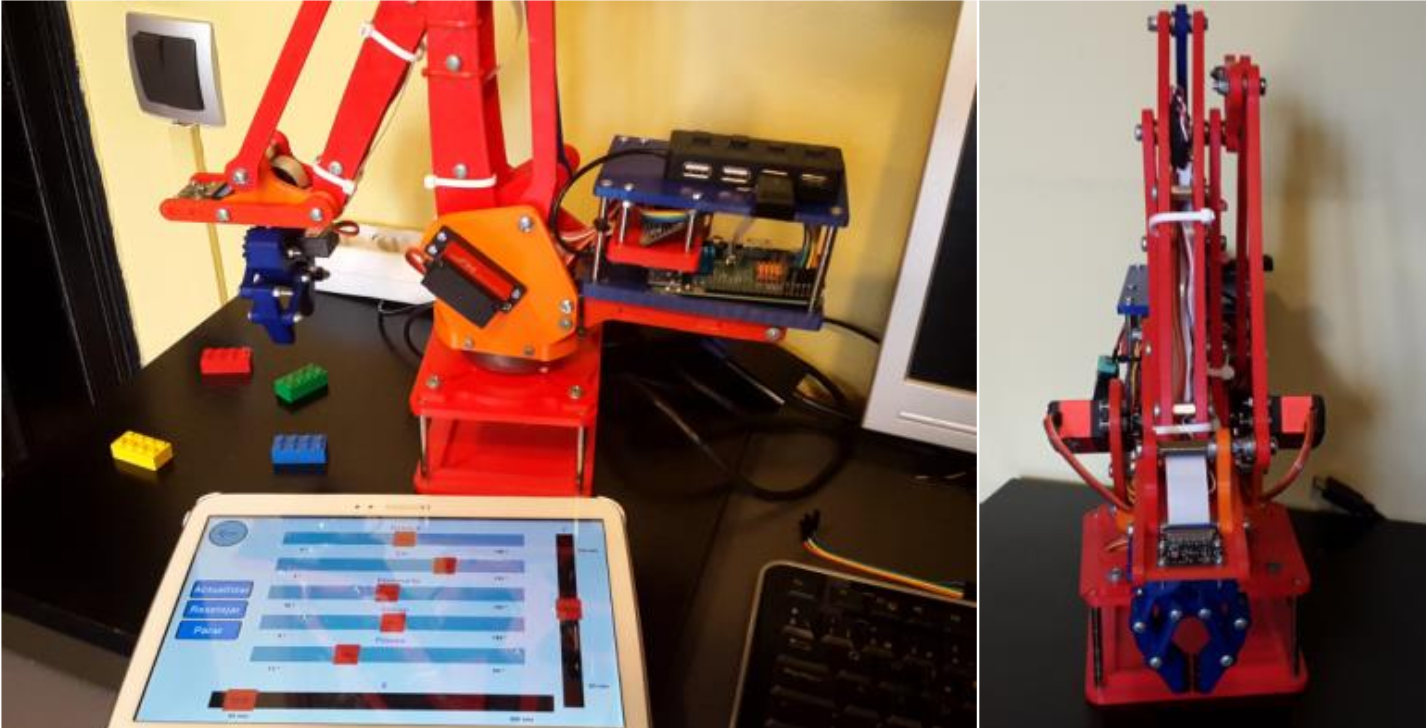
\includegraphics[width = \textwidth]{Robot.png}
    \end{figure}
    \begin{figure}
      \centering
      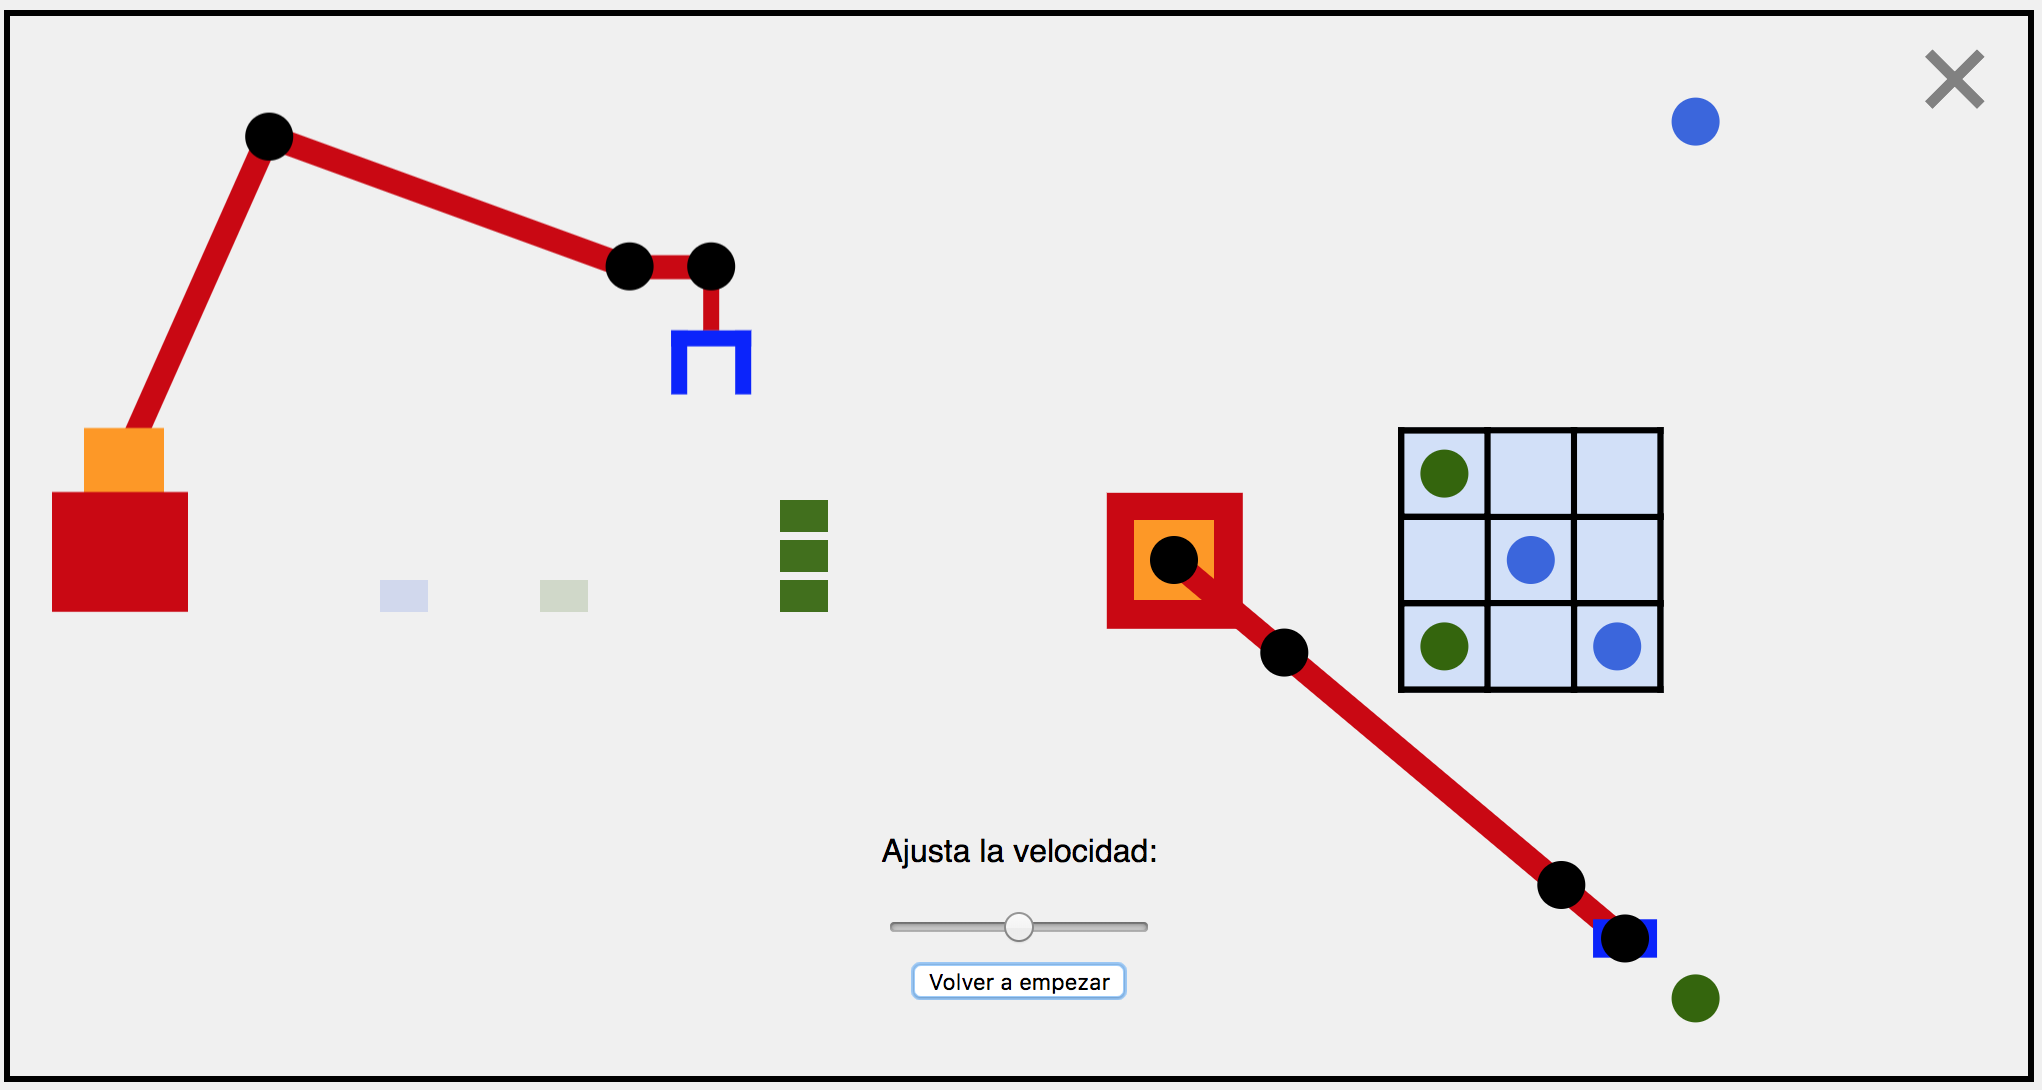
\includegraphics[width = \textwidth]{Animacion.png}
    \end{figure}
  \end{columns}
\end{frame}

\begin{frame}{Replanteamiento del proyecto}
  \begin{figure}
      \centering
      
\includegraphics[width=.7\textwidth]{worldwideweb.png}
  \end{figure}

\end{frame}


\section{Herramientas e implementación}

\subsection{Introducción}

\begin{frame}{Herramientas e implementación}
  \begin{itemize}
    \item ¿Qué herramientas se han usado en este proyecto?
    \item ¿Qué lenguajes de programación se han usado?
  \end{itemize}
\end{frame}

\subsection{Tres en Raya}

\begin{frame}{Lenguaje de programación Tres en Raya}
  \begin{columns}
    \column{.7\textwidth}
    \begin{itemize}
      \item Python como lenguaje principal.
      \item Bibliotecas usadas:
      \begin{itemize}
        \item Random $\rightarrow$ Aleatorizar movimientos.
        \item Sys $\rightarrow$ Leer variables desde terminal.
        \item Math $\rightarrow$ Resolución de ecuaciones de enlace.
        \item \colorbox{gray!50}{Adafruit} $\rightarrow$ Mover servos.
        \item \colorbox{gray!50}{Time} $\rightarrow$ Sleep.
        \item \colorbox{gray!50}{Threading} $\rightarrow$ Movimiento simultáneo.
      \end{itemize}
    \end{itemize}
    \column{.3\textwidth}
    \begin{figure}
      \centering
      
\includegraphics[width = \textwidth]{Logo_Python.png}
    \end{figure}
  \end{columns}

  \note{
    Comentar que \underline{solo} se han usado librerías básicas, todo lo demás
    lo hemos hecho nosotros. \\
    Las librerías que están subrayadas son las que se usarían si estuviera
    funcionando el brazo robótico (nosotros en la web no las usamos).
  }
\end{frame}


\subsection{Servidor web}

\begin{frame}{El servidor web usado y lenguajes}
  \begin{columns}
    \column{.55\textwidth}
    \begin{itemize}
      \item Servidor Web usado: Apache.
      \begin{itemize}
        \item Software libre.
        \item Es el servidor web más usado actualmente en el mundo.
      \end{itemize}
      \item Lenguaje usado para conectar el servidor web con el código en
      Python: PHP.
    \end{itemize}
    \column{.4\textwidth}
    \begin{figure}
      \centering
      
\includegraphics[width = \textwidth]{Logo_Apache.png}
    \end{figure}
    \begin{figure}
      \centering
      
\includegraphics[width = \textwidth]{Logo_PHP.png}
    \end{figure}
  \end{columns}
\end{frame}


\subsection{Interfaz gráfica}

\begin{frame}{Lenguajes utilizados en la Interfaz}
  \begin{itemize}
    \item \underline{HTML}: Creación de la estructuración de la web.
    \item \underline{CSS}: Hojas de estilo (apariencia de la web).
    \item \underline{JS}: Animación del brazo robótico.
  \end{itemize}
  \vspace{.75cm}
  \begin{figure}[b]
    \centering
    
\includegraphics[width = .2\textwidth]{Logo_HTML.png}
    \hspace{.1\textwidth}
    
\includegraphics[width = .2\textwidth]{Logo_CSS.png}
    \hspace{.1\textwidth}
    
\includegraphics[width = .2\textwidth]{Logo_JS.png}
  \end{figure}
\end{frame}


\subsection{Resumen}

\begin{frame}{Resumen de lenguajes utilizados}
\begin{table}[htbp]
  \centering
  \renewcommand{\arraystretch}{1.25}
  \setlength{\tabcolsep}{1.5\tabcolsep}
  \rowcolors{2}{white}{gray!30}
  \begin{tabular}{*3c}
    \toprule
    Lenguaje & \# Archivos & \# Líneas total \\
    \midrule
    Python \imgInline{Logo_Python.png} & 9 & 1025 \\
    JavaScript \imgInline{Logo_JS.png} & 2 & 366 \\
    PHP \imgInline{Logo_PHP.png} + HTML \imgInline{Logo_HTML.png} & 18 & 1315 \\
    CSS \imgInline{Logo_CSS.png} & 3 & 696 \\
    \hline
    TOTAL & 32 & 3402 \\
    \bottomrule
  \end{tabular}
  \vspace{1cm}
  \begin{itemize}
    \item Otros: \LaTeX para presentaciones (Beamer), gráficos e informe.
  \end{itemize}
\end{table}
\end{frame}


\section{Funcionamiento y lógica}

\begin{frame}{Funcionamiento y lógica}
  \begin{itemize}
    \item ¿Cuál es la lógica detrás de la estrategia del Tres en Raya?
    \item ¿Cómo se mueven las piezas?
    \item ¿Cómo funciona la animación?
  \end{itemize}
\end{frame}


\subsection{Tres en Raya}

\begin{frame}{Funcionamiento estrategia Tres en Raya}
  \begin{itemize}
    \item Provee una respuesta al input proporcionado
    \item Juego suma cero $\Rightarrow$ con una estrategia correcta se puede evitar perder
    \item Desarrollo del árbol de posibilidades, evitando las ramas perdedoras
    \item \textbf{FINALIDAD:} Dado un tablero, ``guiar'' la partida hacia una
    posición ganadora o acabar en tablas mediante una \textit{estrategia
      básica.}
  \end{itemize}
\end{frame}

\begin{frame}{Descarte de tableros según simetrías}
  \begin{columns}
    \column{0.5\textwidth}
    \begin{figure}
      \centering
      \scalebox{.5}{% -*- TeX-master: "Presentación.tex" -*-


% Simetrías.

\begin{tikzpicture}
  \node[board, draw] (R) {
    \x \& \e \& \e \\
    \e \& \e \& \e \\
    \e \& \e \& \e \\
  };
  \node[board, right = of R] (A) {
    \x \& \o \& \e \\
    \e \& \e \& \e \\
    \e \& \e \& \e \\
  };
  \node[board, right = of A] (B) {
    \x \& \e \& \o \\
    \e \& \e \& \e \\
    \e \& \e \& \e \\
  };
  \node[board, below = of R] (C) {
    \x \& \e \& \e \\
    \o \& \e \& \e \\
    \e \& \e \& \e \\
  };
  \node[board, below = of A] (D) {
    \x \& \e \& \e \\
    \e \& \o \& \e \\
    \e \& \e \& \e \\
  };
  \node[board, below = of B] (E) {
    \x \& \e \& \e \\
    \e \& \e \& \o \\
    \e \& \e \& \e \\
  };
  \node[board, below = of C] (F) {
    \x \& \e \& \e \\
    \e \& \e \& \e \\
    \o \& \e \& \e \\
  };
  \node[board, below = of D] (G) {
    \x \& \e \& \e \\
    \e \& \e \& \e \\
    \e \& \o \& \e \\
  };
  \node[board, below = of E] (H) {
    \x \& \e \& \e \\
    \e \& \e \& \e \\
    \e \& \e \& \o \\
  };
  \pause
  \draw[<->, ultra thick] (A-3-1.south west) to node[right]{Simetría}
  (C-1-3.north east);
  \draw[<->, ultra thick] (B-3-1.south west) to node[right, very near
  start]{Simetría} (F-1-3.north east);
  \draw[<->, ultra thick] (E-3-1.south west) to node[right]{Simetría}
  (G-1-3.north east);
  \cross{C}
  \cross{F}
  \cross{G}
\end{tikzpicture}
}
    \end{figure}
    \column{0.3\textwidth}
    \begin{itemize}
      \item Permite pasar de $9!$ (362800) tableros a 30.
    \end{itemize}
  \end{columns}
\end{frame}

\begin{frame}{Estrategia básica}
  \begin{columns}
    \column{0.6\textwidth}
    \begin{figure}
      \centering
      \scalebox{.5}{
        \begin{tikzpicture}[tree]
          \node[board] (20) {
            \o \& \e \& \e \\
            \o \& \e \& \x \\
            \e \& \e \& \x \\
          }
          child {
            node[board] (21) {
              \o \& \e \& \e \\
              \o \& \e \& \x \\
              \x \& \e \& \x \\
            }
          }
          child {
            node[board] (22) {
              \o \& \e \& \x \\
              \o \& \e \& \x \\
              \e \& \e \& \x \\
            }
          };
          % \draw[marker = RoyalBlue] (1-1-1.north west) to (1-3-3.south east);
          \draw[marker = OliveGreen] (22-3-3.south) to (22-1-3.north);
          % \draw[marker = OliveGreen] (22-2-1.west) to (22-2-3.east);
          % \draw[marker = RoyalBlue] (23-1-1.north) to (23-3-1.south);
        \end{tikzpicture}
      }
    \end{figure}
    \column{0.4\textwidth}
    \begin{itemize}
      \item \textbf{NO} es suficiente para evitar la derrota.
    \end{itemize}
  \end{columns}
\end{frame}

\begin{frame}{Una rama como ejemplo}
  \begin{figure}
    \centering
    \vspace{-1.25cm}
    \scalebox{.375}{% -*- TeX-master: "Informe.tex" -*-

\begin{tikzpicture}[tree]
  \node[board] {
    \o \& \e \& \e \\
    \e \& \e \& \e \\
    \e \& \e \& \e \\
  }
  child {
    node[board] {
      \o \& \e \& \e \\
      \e \& \x \& \e \\
      \e \& \e \& \e \\
    }
    child {
      node[board] {
        \o \& \o \& \e \\
        \e \& \x \& \e \\
        \e \& \e \& \e \\
      }
      \EB
    }
    child {
      node[board] {
        \o \& \e \& \o \\
        \e \& \x \& \e \\
        \e \& \e \& \e \\
      }
      \EB
    }
    child {
      node[board] {
        \o \& \e \& \e \\
        \e \& \x \& \o \\
        \e \& \e \& \e \\
      }
      child{
        node[board] {
          \o \& \e \& \e \\
          \e \& \x \& \o \\
          \x \& \e \& \e \\
        }
      }
      \EB
    }
    child {
      node[board] {
        \o \& \e \& \e \\
        \e \& \x \& \e \\
        \e \& \e \& \o \\
      }
      child {
        node[board] {
          \o \& \x \& \e \\
          \e \& \x \& \e \\
          \e \& \e \& \o \\
        }
      }
      \EB
    }
  };
\end{tikzpicture}
}
  \end{figure}
\end{frame}


\subsection{Interfaz gráfica}

\begin{frame}{Interfaz gráfica}
  \begin{columns}
    \column{.55\textwidth}
    \begin{itemize}
      \item Se trata de una interfaz web.
      \item Juego de Tres en Raya interactivo.
      \item Información de ángulos.
      \item Documentación y código dentro de la web.
    \end{itemize}
    \column{.45\textwidth}
    \begin{figure}
      \centering
      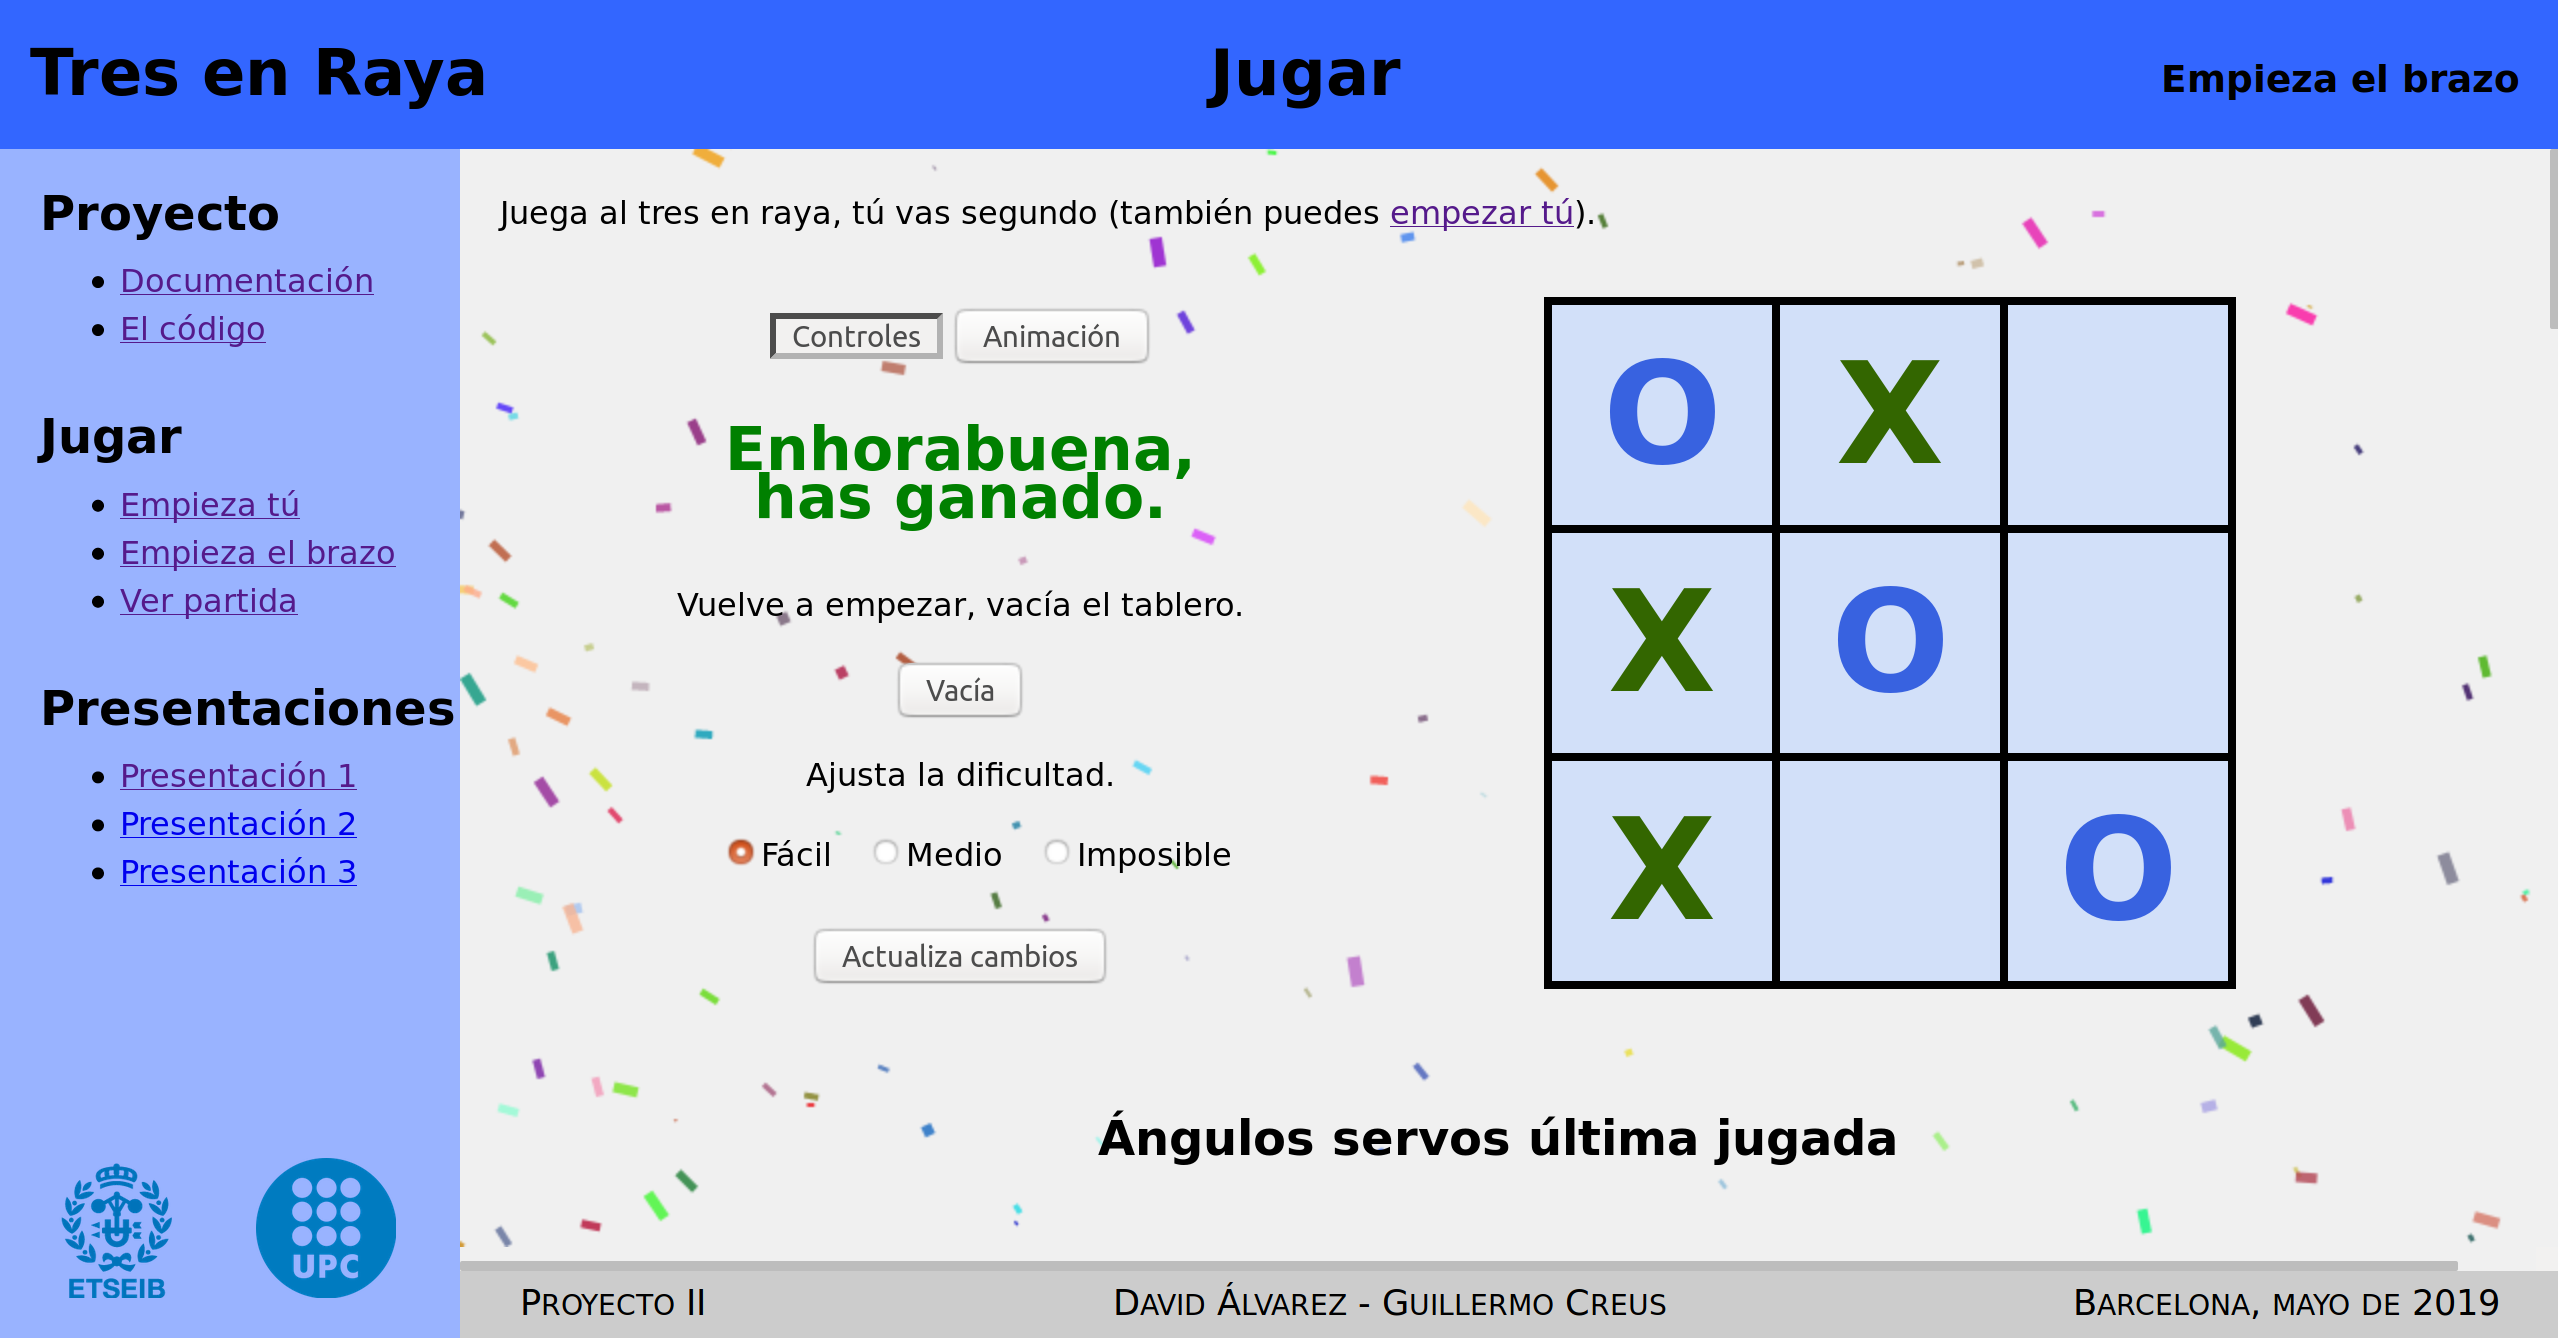
\includegraphics[width = \textwidth]{Interfaz_web.png}
    \end{figure}
    \begin{figure}
      \centering
      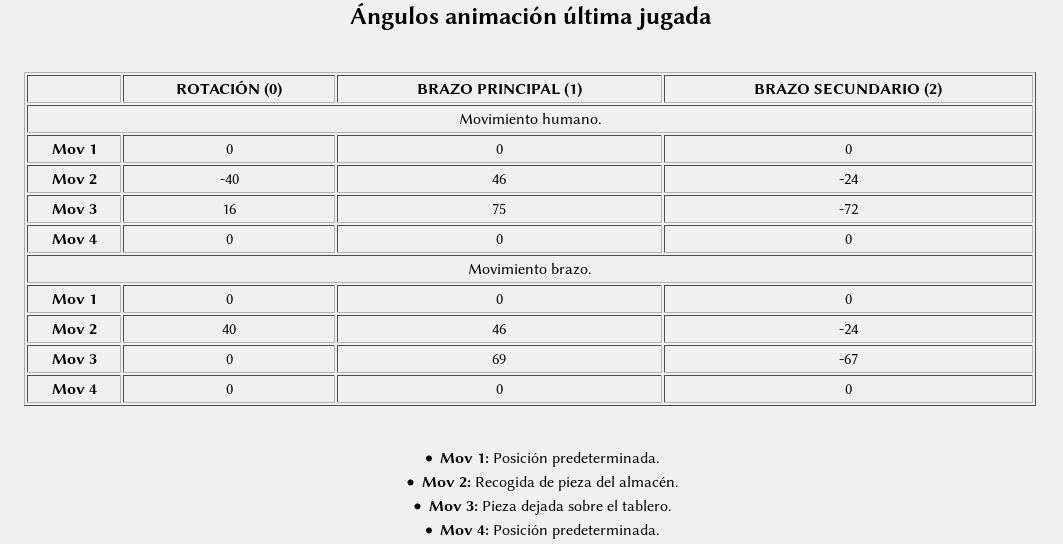
\includegraphics[width = \textwidth]{Interfaz_tabla.png}
    \end{figure}
  \end{columns}
\end{frame}

\begin{frame}{Servidor web}
  \begin{figure}
    \centering
    \scalebox{.65}{% -*- TeX-master: "Informe.tex" -*-

\begin{tikzpicture}
  % Cliente.
  \node[boxp = magenta] (Us) {Usuario};
  \node[box = magenta] (UN) [right = of Us] {Navegador};
  \begin{scope}[on background layer]
    \node[fit = (Us)(UN), cont = magenta, label = {Cliente}] (U) {};
  \end{scope}

  % Servidor Web.
  \node[boxp = gray] (SI) [below = 1.25 of U, xshift = -6.5] {\textit{Index}};
  \node[box = gray] (ST) [left = .75 of SI] {Tablero};
  \node[box = gray] (SN) [right = .75 of SI] {\textit{Navbar}};
  \node[box = gray] (SD) [below = .5 of ST] {Data};
  \node[box = gray] (SA) [right = .35 of SD] {Animación};
  \node[box = gray] (SC) [below = .5 of SN] {Controles};
  \node[box = gray] (SCi) [below = .5 of SD] {Animación};
  \node[box = gray] (SF) [below = .5 of SA, xshift = .25cm] {\textit{Footer}};
  \node[box = gray] (SE) [below = .5 of SC, xshift = .55cm] {Otros \ldots};
  \begin{scope}[on background layer]
    \node[fit = (SI)(ST)(SN)(SC)(SCi)(SD)(SE)(SA), cont = gray,
    label = above right:{Servidor Web}] (S) {};
  \end{scope}

  % Programa Principal.
  \node[boxp = orange] (Mai) [below = 1.5 of S] {Main};
  \begin{scope}[on background layer]
    \node[fit = (Mai), cont = orange, label = below:{Programa principal}] (Ma) {};
  \end{scope}

  % Brazo robótico.
  \node[boxp = red] (MM) [above right = .25 and 4 of Ma] {Principal};
  \node[box = red] (MP) [below = .5 of MM] {Plano};
  \node[box = red] (MI) [below = .5 of MP] {Interpolación};
  \begin{scope}[on background layer]
    \node[fit = (MM)(MP)(MI), cont = red, label = {Movimiento robot}] (M) {};
  \end{scope}

  % Tres en Raya.
  \node[boxp = blue] (TEs) [above left = .78 and 4 of Ma] {Principal};
  \node[box = blue] (TB) [below = .5 of TEs] {Básica};
  \node[box = blue] (TEq) [below = .5 of TB] {Equivalencias};
  \node[box = blue] (TA) [below = .5 of TEq] {Auxiliar};
  \begin{scope}[on background layer]
    \node[fit = (TEs)(TB)(TEq)(TA), cont = blue, label = {Estrategia Tres en Raya}] (T) {};
  \end{scope}

  % Conexiones globales.
  \connectV{U}{S};
  \connectV{S}{Ma};
  \connectH{T}{Ma};
  \connectH{Ma}{M};
\end{tikzpicture}
}
  \end{figure}
\end{frame}


\subsection{Movimiento}

\begin{frame}{Brazo robótico virtual a escala}
  \begin{columns}
    \column{.6\textwidth}
    \begin{enumerate}
      \item Definición puntos en el espacio de almacen.
      \item Resolución de ecuaciones de enlace cinemáticas (coordenadas $\rightarrow$
      ángulos).
      \item JS mueve las barras.
      \item Definición puntos en el espacio de posición en el tablero.
      \item Igual que (2).
    \end{enumerate}
    \column{.4\textwidth}
    \begin{figure}
      \centering
      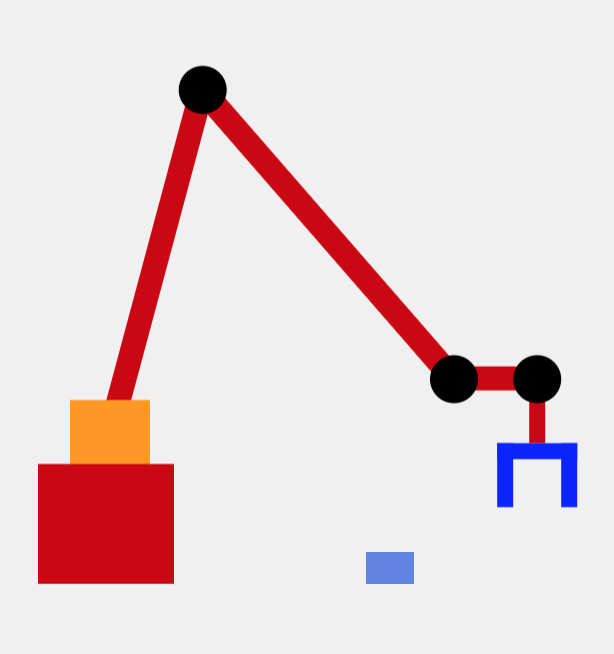
\includegraphics[width = \textwidth]{Brazo_escala.png}
    \end{figure}
  \end{columns}
\end{frame}

\begin{frame}{Brazo robótico virtual a escala II}
  \begin{figure}
    \centering
    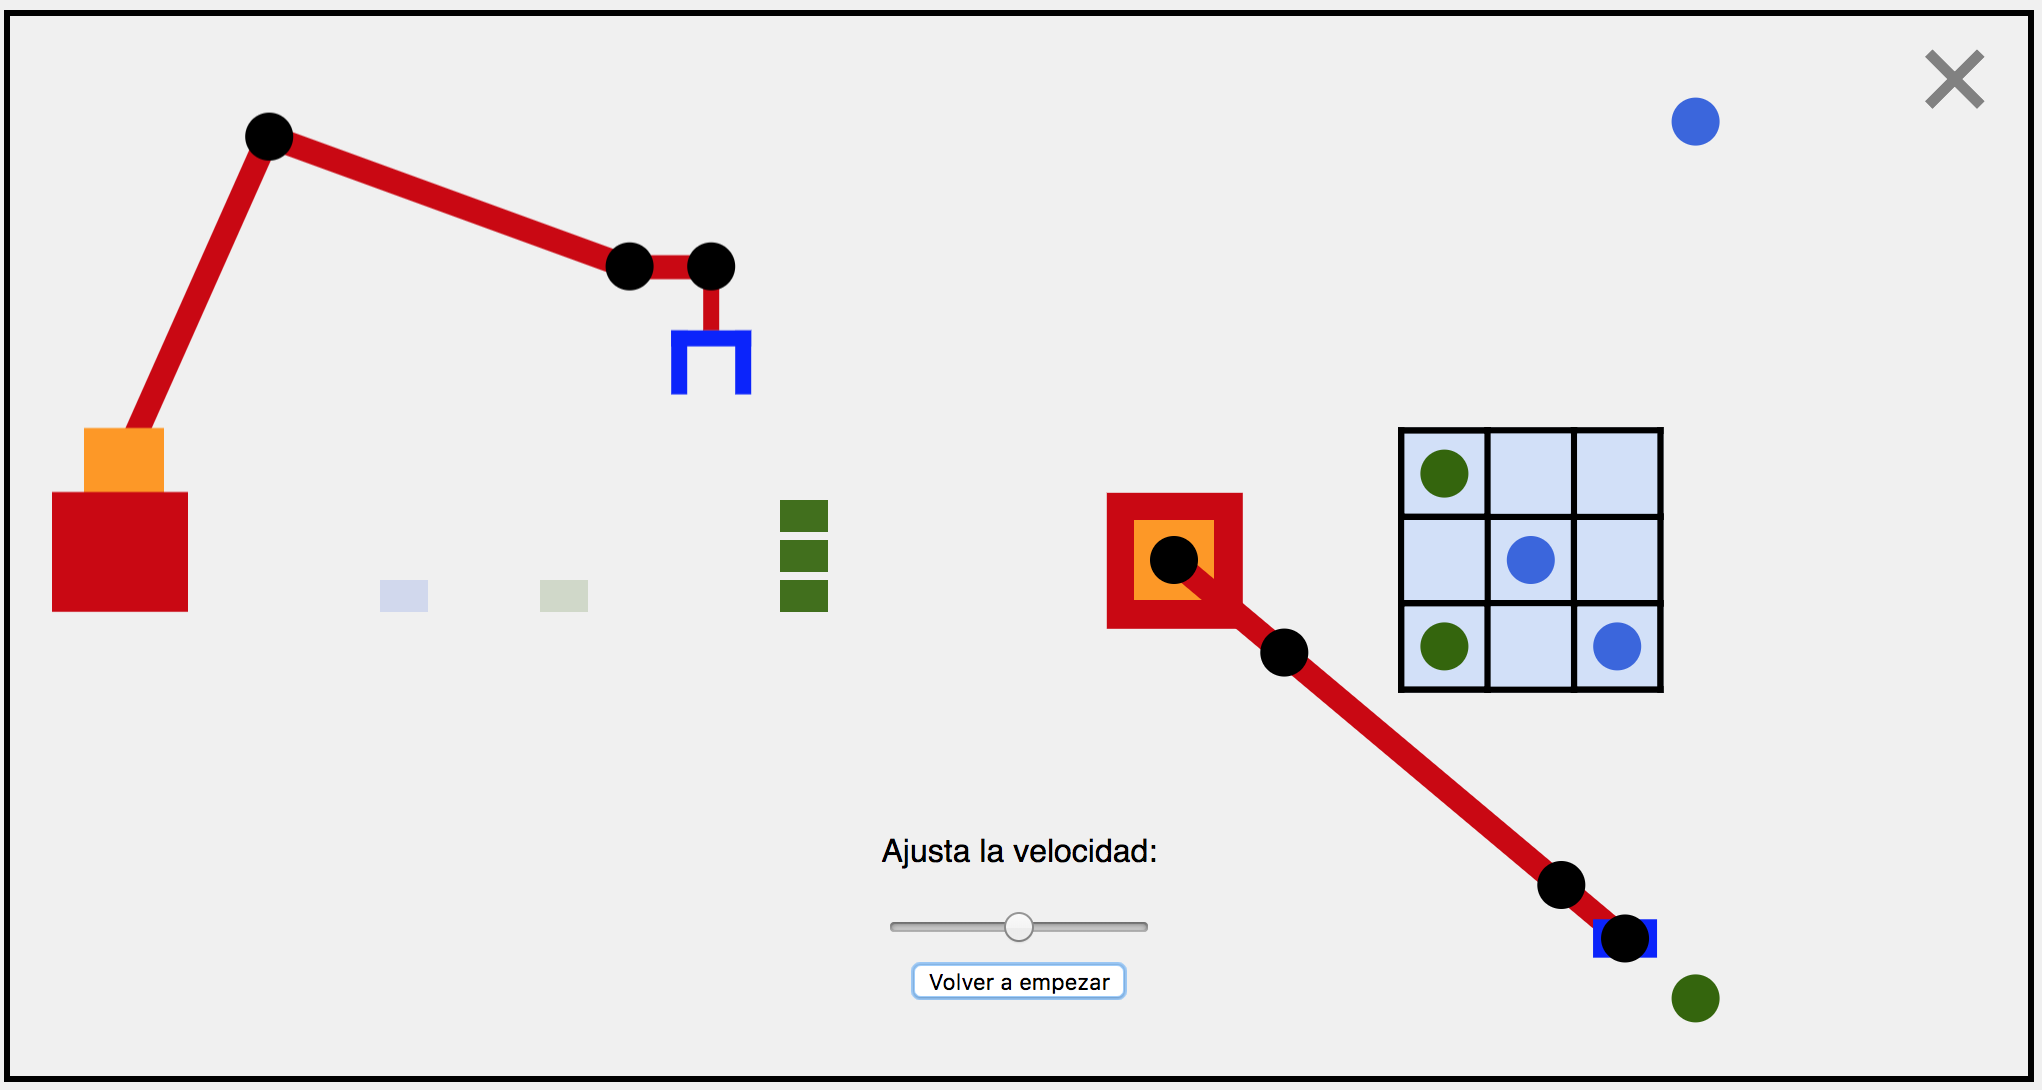
\includegraphics[width = .95\textwidth]{Animacion.png}
  \end{figure}
  \note{
    Comentar la simultaneidad de movimientos. \\
    La velocidad se puee ajustar también.
  }
\end{frame}


\section{Demostración}

\subsection{Resultados}

\begin{frame}{Resultados}
  \begin{center}
    \href{https://alvarezrosa.com/proyecto/}{Comenzar}
  \end{center}
  \note{
    Clicamos y enseñamos la web.
  }
\end{frame}


\end{document}
